\section{Local}
A residência estudada se localiza na Região do Riacho Fundo I, com um tamanho de 160 metros quadrados, atendendo todas as especificações do projeto.

\subsection{A casa}
\par A casa segue a idéia inicial, de uma casa pronta e com toda sua estrutura pré definida. Seus cômodos são: sala, cozinha, quartos, banheiros, escritório, garagem, área de serviço e varanda.
\par A composição da casa é dada da seguinte maneira:
\par \textbf{Paredes:}
    \begin{itemize}
        \item Reboco, tipo de argamassa para deixar as paredes uniformes e aptas a receber a tinta;
        \item Tinta Pva látex, a base de acetato de polivinila, uma tinta solúvel em água de fácil utilização e facilmente encontrada no mercado;
        \item Azulejo, material cerâmico utilizado para revestir pisos e paredes, impermeável e facilmente limpável.
    \end{itemize}
\par \textbf{Pisos:}
    \begin{itemize}
        \item Azulejo, material cerâmico utilizado para revestir pisos e paredes, impermeável e facilmente limpável.
    \end{itemize}
\subsection{Planta baixa e desenho da casa}

\begin{center}
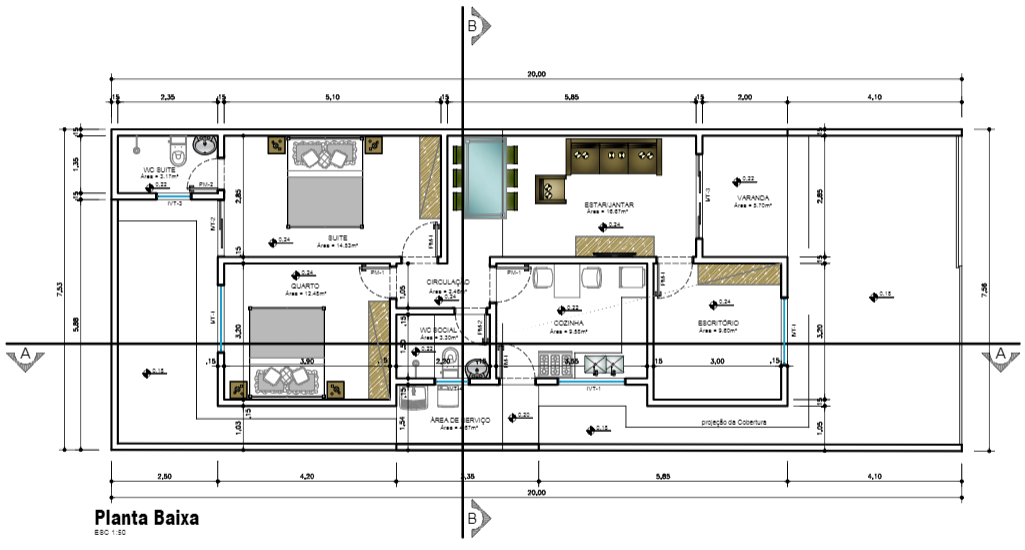
\includegraphics[width=\textwidth]{figuras/planta}
\end{center}

\begin{center}
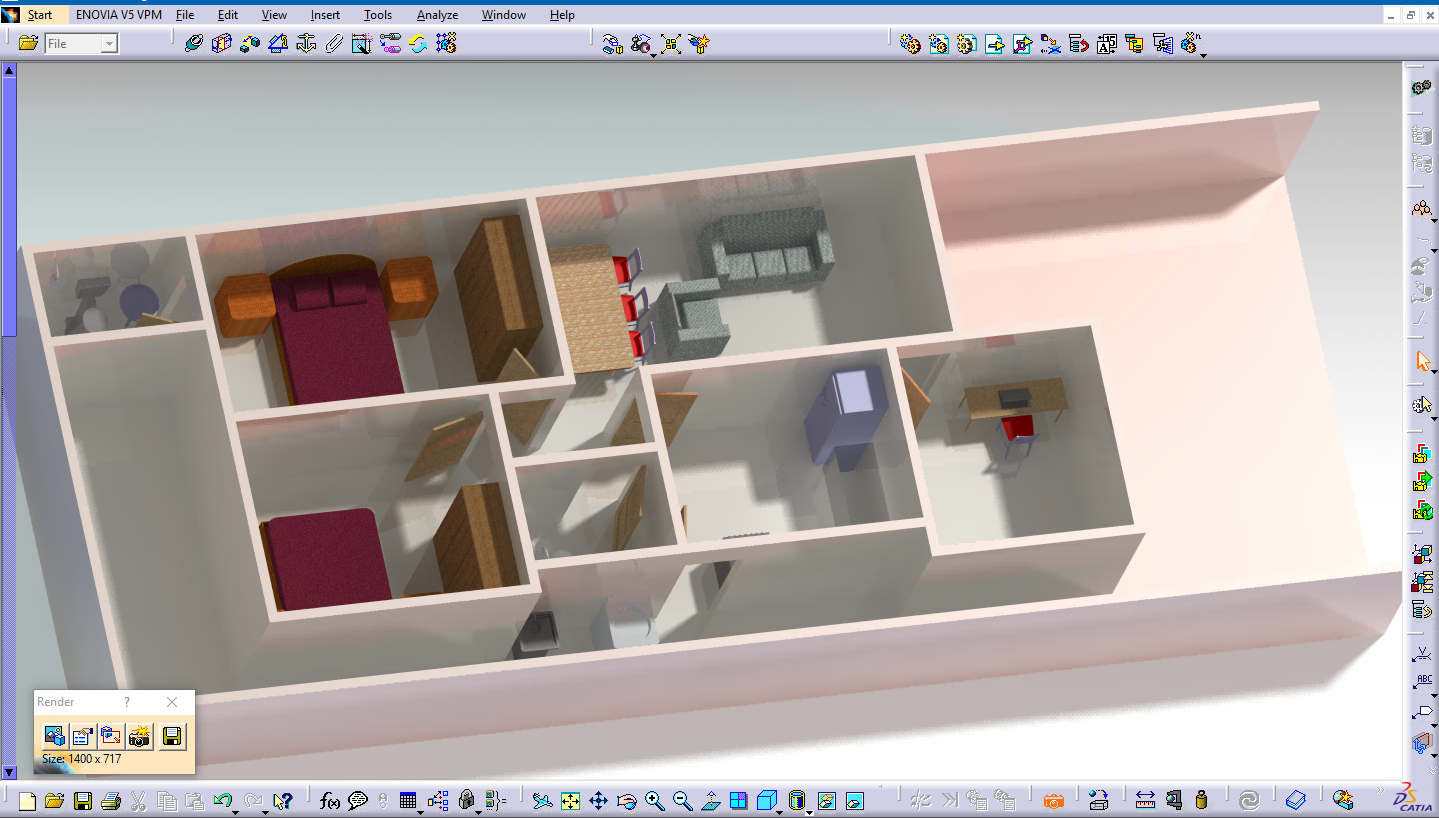
\includegraphics[width=\textwidth]{figuras/modelo3D}
\end{center}
